% Asset ID: AS1AlgebraicMethodsProofTikZ-003
% Source: Chapter 7b Algebraic Methods, Proof transcript
% Related lesson section: Key Definitions and Notation
% Purpose: Algebraic forms reference card for proof.

\documentclass[tikz,border=8pt]{standalone}
\usepackage{amsmath}
\usetikzlibrary{positioning}
\begin{document}
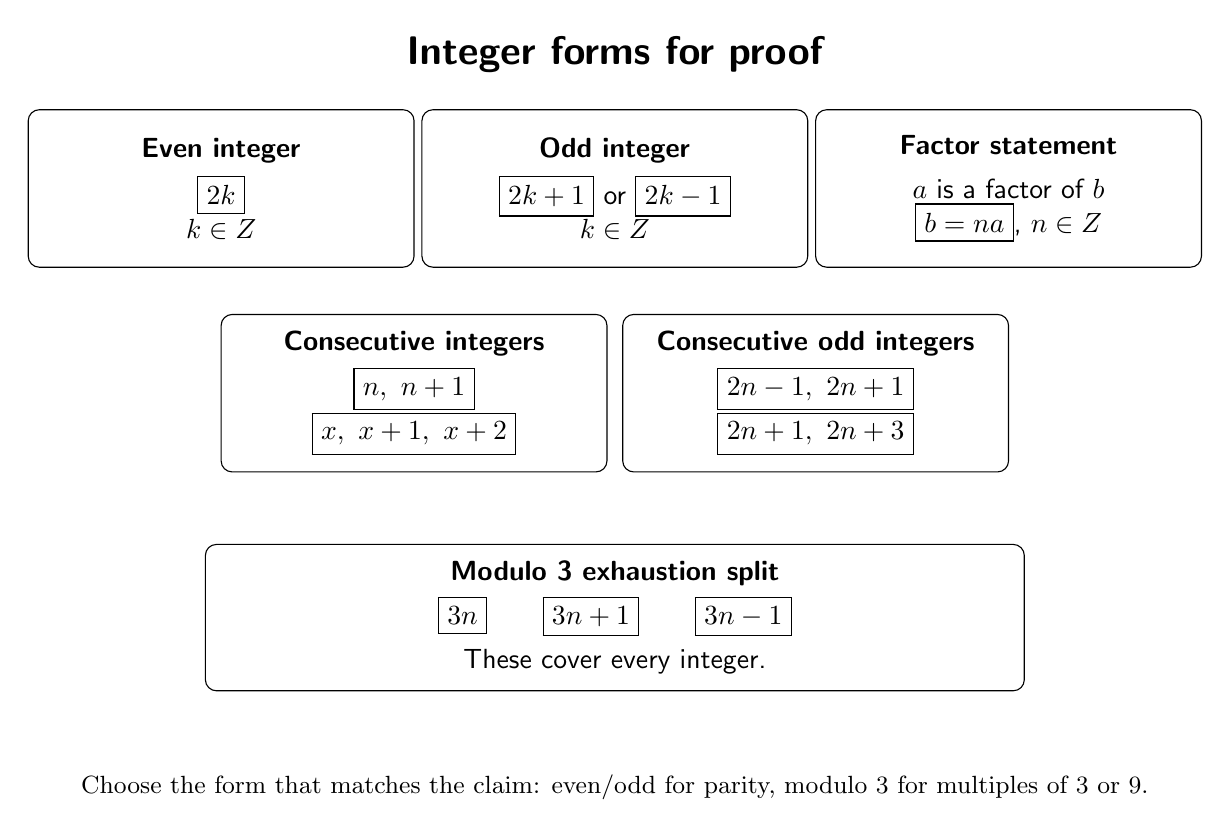
\begin{tikzpicture}[font=\sffamily,card/.style={draw,rounded corners,align=center,minimum width=4.9cm,minimum height=2.0cm,inner sep=6pt},wide/.style={draw,rounded corners,align=center,minimum width=10.4cm,minimum height=1.75cm,inner sep=6pt}]
\node[font=\sffamily\bfseries\Large, align=center] at (0,5.3){Integer forms for proof};
\node[card] at (-5,3.6){\textbf{Even integer}\\[4pt]\(\boxed{2k}\)\\\(k\in\mathbb Z\)};
\node[card] at (0,3.6){\textbf{Odd integer}\\[4pt]\(\boxed{2k+1}\) or \(\boxed{2k-1}\)\\\(k\in\mathbb Z\)};
\node[card] at (5,3.6){\textbf{Factor statement}\\[4pt]\(a\) is a factor of \(b\)\\\(\boxed{b=na}\), \(n\in\mathbb Z\)};
\node[card] at (-2.55,1.0){\textbf{Consecutive integers}\\[4pt]\(\boxed{n,\ n+1}\)\\\(\boxed{x,\ x+1,\ x+2}\)};
\node[card] at (2.55,1.0){\textbf{Consecutive odd integers}\\[4pt]\(\boxed{2n-1,\ 2n+1}\)\\\(\boxed{2n+1,\ 2n+3}\)};
\node[wide] at (0,-1.85){\textbf{Modulo 3 exhaustion split}\\[4pt]\(\boxed{3n}\qquad \boxed{3n+1}\qquad \boxed{3n-1}\)\\[4pt]These cover every integer.};
\node[align=center, font=\small] at (0,-4){Choose the form that matches the claim: even/odd for parity, modulo 3 for multiples of \(3\) or \(9\).};
\end{tikzpicture}
\end{document}
